\documentclass[11pt, oneside]{article}   	% use "amsart" instead of "article" for AMSLaTeX format
\usepackage[a4paper, total={7in, 9in}, margin=0.5in]{geometry}                		% See geometry.pdf to learn the layout options. There are lots.
\geometry{letterpaper}                   		% ... or a4paper or a5paper or ... 
%\geometry{landscape}                		% Activate for for rotated page geometry
\usepackage[parfill]{parskip}    		% Activate to begin paragraphs with an empty line rather than an indent
\usepackage{graphicx}				% Use pdf, png, jpg, or eps§ with pdflatex; use eps in DVI mode
								% TeX will automatically convert eps --> pdf in pdflatex	
\graphicspath{ {./images/} }

\usepackage{amsmath}
\usepackage{amssymb}
\usepackage{subfig}
\usepackage{floatrow}
% Table float box with bottom caption, box width adjusted to content
\newfloatcommand{capbtabbox}{table}[][\FBwidth]
\usepackage{float}
%\usepackage{caption}
%\usepackage{subcaption}
\usepackage{nicefrac}
\usepackage{mathtools}
\usepackage{amssymb}

    
%\setcounter{section}{2}

\title{MANIP Lab report (M1 CORO/JEMARO)}
\author{Joseph Webb\quad - \quad Thursday 17 November 2022}
\date{}							% Activate to display a given date or no date

\begin{document}

\maketitle
\section{Modified DH-Tables}

\subsection{Turret Robot}

$r_1 = 0.5, \quad r_2 = 0.1$


\begin{figure}[H]
\begin{floatrow}
\ffigbox{%
  %\rule{3cm}{3cm}%
%}
%{%
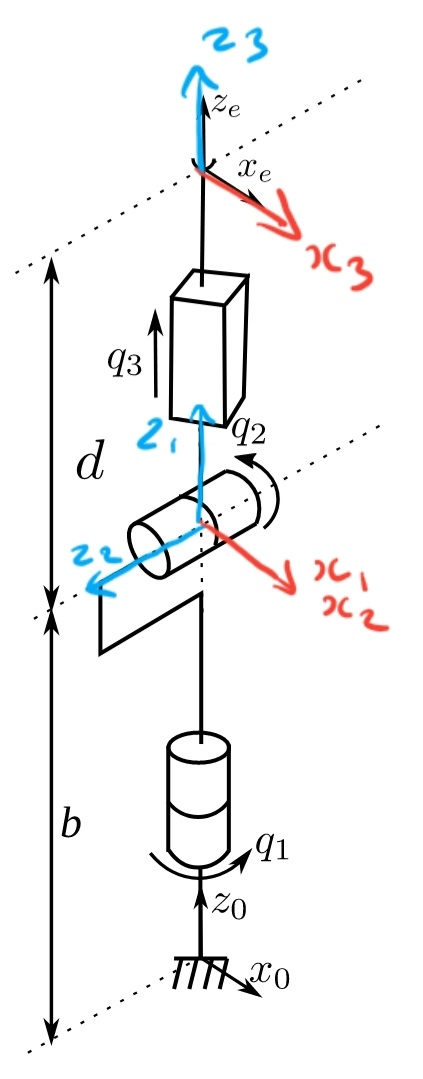
\includegraphics[scale = 0.25]{Turret}
}{%
  \caption{schematic of turret robot with intermediary frames}%
}
\capbtabbox{%
  \begin{tabular}{ | c | c  c  c  c |}
\hline
 Joint & a & $\alpha$ & $\theta$ & r \\ 
 \hline
 1 & 0 & 0 &  $q_1$ & b \\ 
 
 2 & 0 & $\nicefrac{\pi}{2}$ & $q_2$ & 0 \\
 
 3 & 0 & $-\nicefrac{\pi}{2}$ & 0 & $ q_3 + d$ \\
 \hline
 e & 0 & 0 & 0 & 0 \\
 \hline

\end{tabular}
}{%
  \caption{Modified DH-table for turret bot}%
}
\end{floatrow}
\end{figure}

\pagebreak

\subsection{KR-16 Robot (KUKA)}

$r_1 = 0.675, \quad r_2 = 0.26, \quad r_3 = 0.68, \quad r_4 = 0.035, \quad r_5 = 0.67, \quad r_e = 0.158$

\begin{figure}[H]
\begin{floatrow}
\ffigbox{%
  %\rule{3cm}{3cm}%
%}
%{%
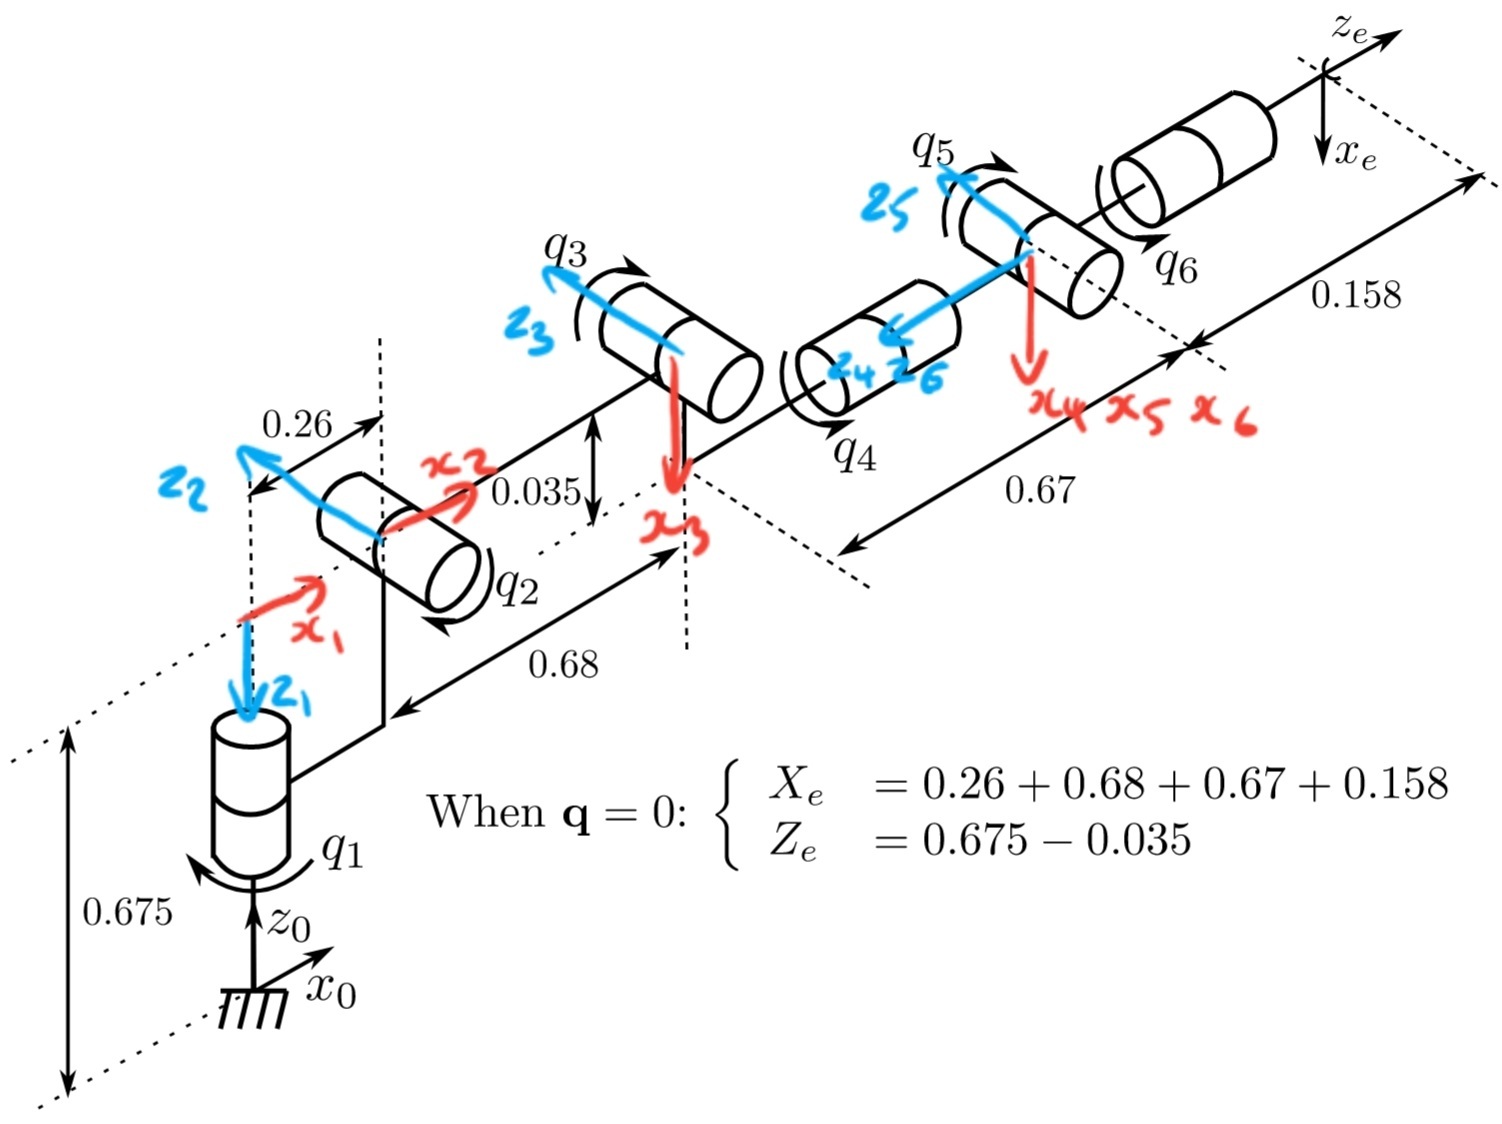
\includegraphics[scale = 0.18]{Kuka}
}{%
  \caption{schematic of KUKA with intermediary frames}%
}
\capbtabbox{%
  \begin{tabular}{ | c | c  c  c  c |}
\hline
 Joint & a & $\alpha$ & $\theta$ & r \\ 
 \hline
 1 & 0 & $\pi$ &  $q_1$ & $-r_1$ \\ 
 
 2 & $r_2$ & $\nicefrac{\pi}{2}$ & $q_2$ & 0 \\
 
 3 & $r_3$ & 0 & $q_3 + \nicefrac{\pi}{2}$ & 0 \\
 
 4 & $r_4$ & $-\nicefrac{\pi}{2}$ & $q_4$ & $-r_5$\\ 
 
 5 & 0 & $\nicefrac{\pi}{2}$ & $q_5$ & 0\\
 
 6 & 0 & $-\nicefrac{\pi}{2}$ & $q_6$ & 0\\
 \hline
 e & 0 & $\pi$ & 0 & $r_e$ \\
 \hline

\end{tabular}
}{%
  \caption{Modified DH-table for KUKA}%
}
\end{floatrow}
\end{figure}

\subsection{UR-10 Robot}

$r_1 = 0.1273, \quad r_2 = 0.612, \quad r_3 = 0.5723, \quad r_4 = 0.1639, \quad r_5 = 0.1157, \quad r_e = 0.1922$

\begin{figure}[H]
\begin{floatrow}
\ffigbox{%
  %\rule{3cm}{3cm}%
%}
%{%
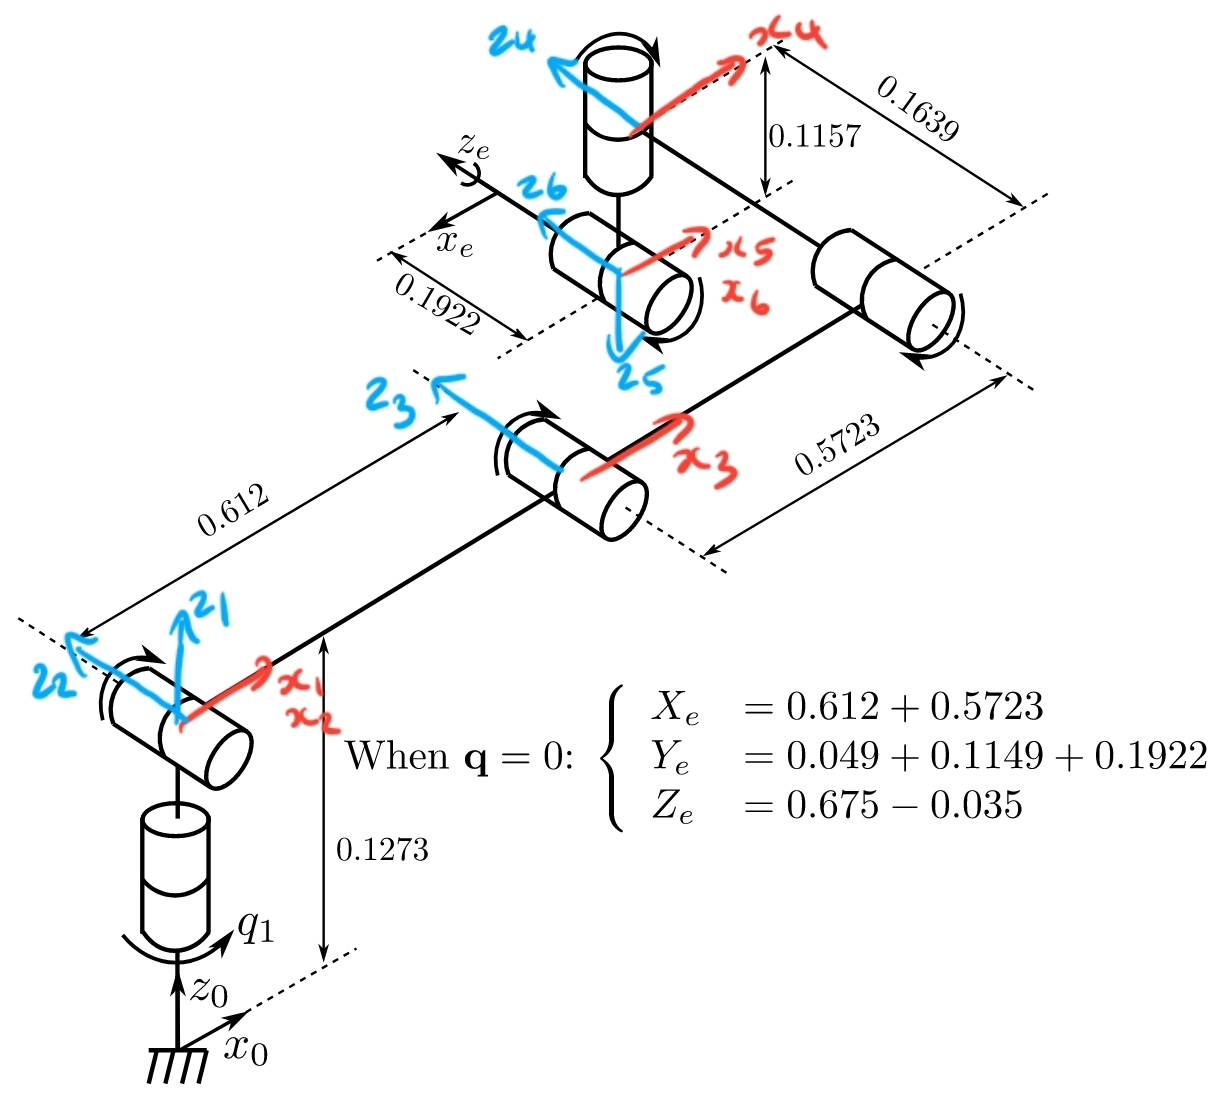
\includegraphics[scale = 0.22]{UR10}
}{%
  \caption{schematic of UR10 with intermediary frames}%
}
\capbtabbox{%
  \begin{tabular}{ | c | c  c  c  c |}
\hline
 Joint & a & $\alpha$ & $\theta$ & r \\ 
 \hline
 1 & 0 & 0 &  $q_1$ & $r_1$ \\ 
 
 2 & 0 & $-\nicefrac{\pi}{2}$ & $q_2$ & 0 \\
 
 3 & $r_2$ & 0 & $q_3$ & 0 \\
 
 4 & $r_3$ & 0 & $q_4$ & $r_4$\\ 
 
 5 & 0 & $-\nicefrac{\pi}{2}$ & $q_5$ & $r_5$\\
 
 6 & 0 & $\nicefrac{\pi}{2}$ & $q_6$ & 0\\
 \hline
 e & 0 & 0 & $\pi$ & $r_e$ \\
 \hline

\end{tabular}
}{%
  \caption{Modified DH-table for UR-10}%
}
\end{floatrow}
\end{figure}

\section{Inverse Geometric Models}

\subsection{Turret Robot}

\begin{equation*}
^fM_w= 
\begin{pmatrix}
c_1 c_2 & -s_1 & -s_2 c_1 & (-q_3 - r_2) s_2  c_1 \\
s_1 c_2& c_1 & -s_1 s_2& (-q_3 - r_2) s_1 s_2 \\
s_2  & 0  & c_2 & r_1 + (q_3 + r_2) c_2  \\
0 & 0 & 0 & 1\\
\end{pmatrix}
=
\begin{pmatrix}
x_x& x_y & x_z & t_x \\
y_x& y_y & y_z & t_y\\
z_x  & z_y  & z_z & t_z  \\
0 & 0 & 0 & 1\\
\end{pmatrix}
\end{equation*}

from $x_y$ and $y_y$ $q_1$ can be computed:

\begin{equation*}
-s_1 = x_y \quad c_1 = y_y
\end{equation*}
\begin{equation}
q_1 = \text{solveType3}(-1,0,y_x,0,1,y_y)
\end{equation}

Then, $q_2$ is solved in the same way:

\begin{equation}
q_2 = \text{solveType3}(1,0,x_z,0,1,z_z)
\end{equation}

Solving for prismatic joint 3 depends on the value of $s_1$ \& $c_1$. If $c_2 \neq 0$ we can use it to solve $q_3$ using the following equation:

\begin{equation}
q_3 = \frac{t_z-r_1}{c_2}-r_2
\end{equation} 

If $c_2 = 0$ but $s_1 \neq 0$ then $s_1$ can be used to solve $q_3$

\begin{equation}
q_3 = -\frac{ty}{s_1 s_2}-r_1
\end{equation}

otherwise, if both are null, the following equation must be used:

\begin{equation}
q_3 = -\frac{t_x}{s_2 c_1}-r_2
\end{equation}

\subsection{KR-16 Robot (KUKA)}

Because of the spherical wrist in the KUKA robot, the IGM can be simplified. First we can calculate the first 3 joint values using the translation between the base frame and the wrist frame. ($t_x,t_y,t_z$)

\begin{equation*}
^{f}t_w = 
\begin{pmatrix}
(a_2 + a_3 c_2 - a_4 s_{23} + r_4 c_{23}) c_1 \\
(-a_2 -a_3 c_2 + a_4 s_{23} -r_4 c_{23}) s_1 \\
-a_3 s_2 - a_4 c_{23} + r_1 - r_4 s_{23}   \\
 1\\
\end{pmatrix}
=
\begin{pmatrix}
t_x\\
t_y\\
t_z\\
1\\
\end{pmatrix}
\end{equation*}



using ${}^ft_w$:

\begin{equation*}
(a_2 + a_3 c_2 - a_4 s_{23} + r_4 c_{23}) = \frac{t_x}{c_1} = -\frac{t_y}{s_1}
\end{equation*}

Therefore, q1 can be solved as

\begin{equation}
q_1 = \text{solveType2}(t_x,t_y,0)
\end{equation}

and the remaining join values can be calculated with a type 7 equation.

\begin{equation}
q_2,q_{23} = \text{solveType7}(0,-a_3,(r_1 - t_z) , (a_2 - \nicefrac{t_x}{c_1}), a_4, r_4)
\end{equation}
\begin{equation}
q_3 = q_{23} - q_2
\end{equation}

Now the rotation can be computed between the wrist frame an the end effector, involving only the last 3 remaining joints. using the equation

\begin{equation*}
P^* = {}^fM_e^* = {}^fM_w{}^wM_e
\end{equation*}

we can compute:

\begin{equation*}
^{0}R_3 = 
\begin{pmatrix}
-s_{23} c_1 & -c_1 c_{23} & s_1 \\
s_1 s_{23} & s_1 c_{23} & c_1 \\
-c_{23} & s_{23} & 0 \\
\end{pmatrix}
\end{equation*}
and
\begin{equation*}
{}^3R_6 = {}^0R_3^{-1}{}^fR_w = 
\begin{pmatrix}
-s_4s_6+c_4c_5c_6 & -s_4c_6-s_6c_4c_5 & -s_5c_4\\
s_5c_6 & -s_5s_6 & c_5\\
-s_4c_5c_6-s_6c_4 & s_4s_6c_5 - c_4c_6 & s_4s_5\\
\end{pmatrix}
=
\begin{pmatrix}
x_x' & y_x' & z_x'\\
x_y' & y_y' & z_y'\\
x_z' & y_z' & z_z'\\
\end{pmatrix}
\end{equation*}

The remaining joints therefore become trivial to solve.

\begin{equation}
q_5 = \text{solveType2}(0,1,z_y')
\end{equation}

\begin{equation}
q_4 = \text{solveType3}(0,-s_5,z_x',s_5,0,z_z')
\end{equation}

\begin{equation}
q_6 = \text{solveType2}(0,s_5,x_y')
\end{equation}




\end{document}  